\newpage\EMPHASIZE{16. Scope}

\textsc{Objectives}

\begin{itemize}
\item
  Understand the scope of a variable
\item
  Understand how C++ searches for a variable
\item
  Understand the importance of using minimal scopes
\end{itemize}

I' ve already mentioned scopes of variables in several
places. In this set of notes, I will collect what you already know about
scopes. So much of it is review. I will also add a few new scope rules.

\newpage\EMPHASIZE{Scope}

A variable has a name, a value, and you should know by now, a variable also has a \EMPHASIZE{scope}. This refers to the place in your code where you can refer to that variable.

Here's an old example (very very very old ...):

\begin{console}
x = 42; // x not declared yet bozo!!!

int x = 0;
std::cout << x << std::endl;
\end{console}

In general the scope of a variable is from the \EMPHASIZE{point of declaration} to the \EMPHASIZE{end of the block where it is declared}. During the execution of the program, when the point of execution exits that block, the variable is destroyed. Try this:

\begin{consolethree}[escapeinside=||]
#include <iostream>

int main()
{   
    int x = 0;
    std::cin >> x;

    if (x == 42)
    {   
       |\tikzmarknode{yboxtl}{}|std::cout << "here we go ..." << std::endl;   |\tikzmarknode{yboxtr}{}|
        int y = x + 1;
        std::cout << "y: " << y << std::endl;        |\tikzmarknode{yboxend}{}|
    }  |\tikzmarknode{yboxbl}{}|                                              |\tikzmarknode{yboxbr}{}||\sidebox{scopeybox}{Scope of y}|
    std::cout << "x: " << x << std::endl;

    return 0;
\end{consolethree}
\DrawArrowPoints[dashed,red,thick]{yboxtr}{yboxend}{-- (yboxtl) -- (yboxbl) -- (yboxbr) -- (yboxtr) -- ++(0,-0.9) -- (scopeybox)}

Of course you should know by now that this won't work (try it):

\begin{consolethree}[escapeinside=||]
#include <iostream>

int main()
{    
     int x = 0;
     std::cin >> x;
     
     if (x == 42)
     {    
          std::cout << "here we go ..." << std::endl;
          int y = x + 1;
          std::cout << "y: " << y << std::endl;
     }
     |\tikzmarknode{badynode}{std::cout << "y: " << y << std::endl;}||\sidebox{badtxbox}{BAD!!!}|

     return 0;
} 
\end{consolethree}
\DrawArrow{badtxbox}{badynode}
\newpage %to keep sideboxes and consoles together on the same page
You should visualize the variables in your code as being created in blocks of memory spaces. Suppose the user enters 42 for \texttt{x} and we are about to execute the print statement in the body of the \texttt{if} statement. The memory looks like this:
%needs some additional direction adjustments, arrows pointing straight down instead of at an angle
%also the boxes are cut off very slightly, the sidenote environment isnt letting me xshift/yshift to correct
\sidenote
{
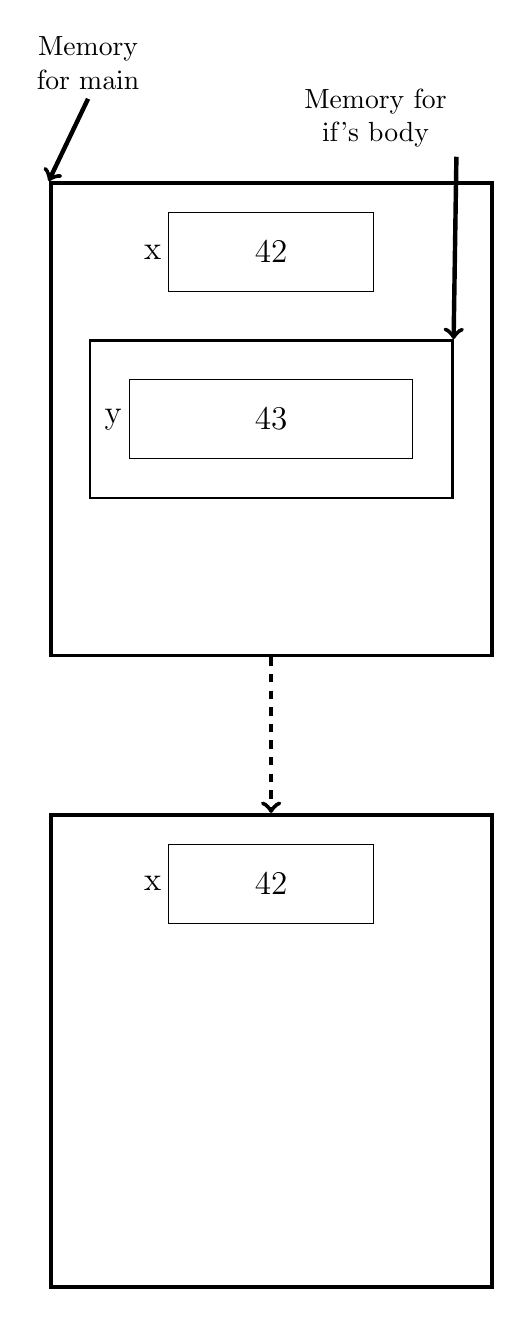
\begin{tikzpicture}
    \node[draw,text width=5cm,minimum height=6cm,minimum width=3cm, line width=0.05cm, inner sep=0.3cm] (a) at (-3,-2) {};
    \node[draw,text width=3cm, minimum height=1cm, line width=0.01cm, inner sep=0.3cm] (b) at (a.center) {};
    \node (fortythree) at (b.center) {\large{43}};
    \node[draw,text width=4cm, minimum height=2cm, line width=0.035cm, inner sep=0.3cm] (c) at (b.center) {};
    \node[draw, yshift=-9mm, text width=2cm, minimum height=1cm, line width=0.01cm, inner sep=0.3cm] (d) at (a.north) {};
    \node[xshift=-2mm] (ymemnode) at (b.west) {\large{y}};
    \node[xshift=-2mm] (xmemnode) at (d.west) {\large{x}};
    \node (fortytwo) at (d.center) {\large{42}};

    \node[xshift=5mm,yshift=15mm, align=center] (memtxtnode) at (a.north west) {\normalsize{Memory} \\ \normalsize{for main}};
    \node[xshift=-15mm, yshift=8mm, align=center] (bdytxtnode) at (a.north east) {\normalsize{Memory for} \\ \normalsize{if's body}};
    
    \draw [ultra thick, ->] (bdytxtnode.south east) to (c.north east);
    \draw [ultra thick, ->] (memtxtnode.south) to (a.north west)[xshift=-5mm];

    \node[draw,text width=5cm,minimum height=6cm,minimum width=3cm, line width=0.05cm, inner sep=0.3cm, yshift=-5cm] (a2) at (a.south) {};

    \draw [ultra thick, dashed, ->] (a.south) to (a2.north);
    
    \node[draw, yshift=-9mm, text width=2cm, minimum height=1cm, line width=0.01cm, inner sep=0.3cm] (d2) at (a2.north) {};
    \node[xshift=-2mm] (xmemnode2) at (d2.west) {\large{x}};
        \node (fortytwo2) at (d2.center) {\large{42}};    
\end{tikzpicture}
}

\begin{consolethree}[escapeinside=||]
#include <iostream>

int main()
{    
     int x = 0;
     std::cin >> x;
     
     if (x == 42)
     {   
         std::cout << "here we go ..." << std::endl;
         int y = x + 1;
         |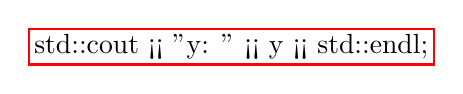
\begin{tikzpicture}\node[draw=red, thick, inner sep=2pt]{std::cout << "y: " << y << std::endl;};\end{tikzpicture}|
     }
     std::cout << "y: " << y << std::endl;

     return 0;
}
\end{consolethree}



\begin{consolethree}[escapeinside=||]
#include <iostream>

int main()
{    
     int x = 0;
     std::cin >> x;

     if (x == 42)
     {   
         std::cout << "here we go ..." <<
         std::endl;
         int y = x + 1;
         std::cout << "y: " << y << std::endl;
     }
     |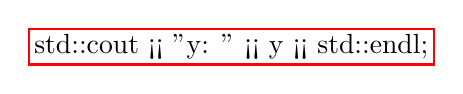
\begin{tikzpicture}\node[draw=red, thick, inner sep=2pt]{std::cout << "y: " << y << std::endl;};\end{tikzpicture}|
             
     return 0;
}
\end{consolethree}
As you can see, immediately on exiting the \texttt{if} statement, the \EMPHASIZE{variable in the body of the \texttt{if} statement is destroyed}.

Of course \texttt{x} was created in the \texttt{main()} block. So \texttt{x} is not destroyed.

This is one of the reasons why proper indentation is so important. Not only does it help you read the logic of your code, it tells you when variables are destroyed.

\newpage\EMPHASIZE{\texttt{for}-loops and \texttt{while}-loops}

You should think of the \texttt{for}-loop as having a block and the body
of the for-loop as having an inner block.
\sidenote
{
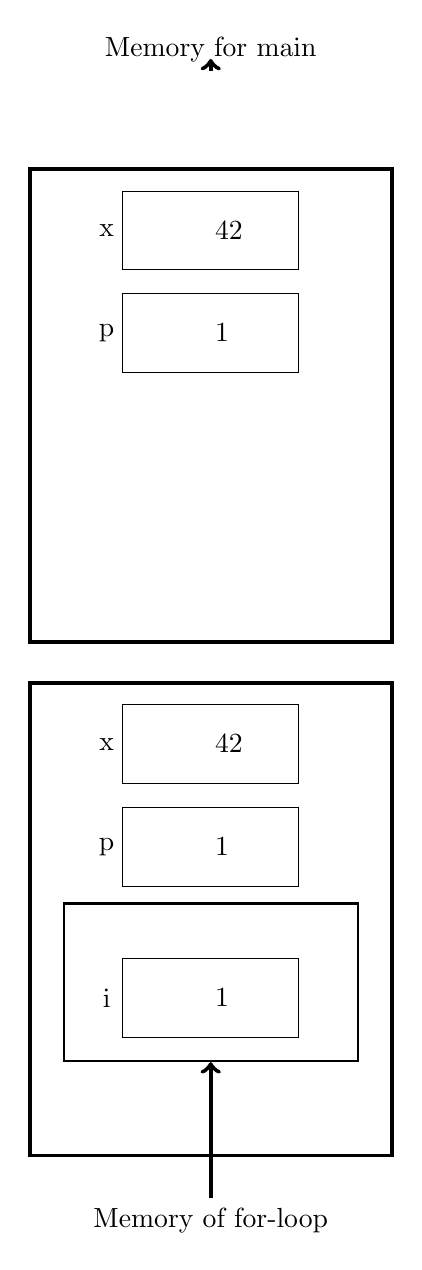
\begin{tikzpicture}
    \node[draw,text width=4cm,minimum height=6cm,minimum width=3cm, line width=0.05cm, inner sep=0.3cm] (fora) at (-3,-2) {};
    \node[draw,text width=2cm,minimum height=1cm,line width=0.01cm,yshift=-8mm] (forxbox) at (fora.north){\normalsize{\texttt{\ \ \ \ \ \ \ \ \ }42}};
    \node[draw,text width=2cm,minimum height=1cm,line width=0.01cm,yshift=-8mm] (forpbox) at (forxbox.south){\normalsize{\texttt{\ \ \ \ \ \ \ \ \ }1}};
    \node[yshift=15mm] (formemnodeanchor) at (fora.north){};
    \node[yshift=15mm] (formemnode) at (fora.north){\normalsize{Memory for main}};
    \node[xshift=-2mm] (forxnode) at (forxbox.west){\normalsize{x}};
    \node[xshift=-2mm] (forpnode) at (forpbox.west){\normalsize{p}};
    \draw[->,ultra thick] (formemnode.south) to (formemnodeanchor);

    \node[draw,text width=4cm,minimum height=6cm,minimum width=3cm, line width=0.05cm, inner sep=0.3cm,yshift=-3.5cm] (for2a) at (fora.south) {};
    \node[draw,text width=2cm,minimum height=1cm,line width=0.01cm,yshift=-8mm] (for2xbox) at (for2a.north){\normalsize{\texttt{\ \ \ \ \ \ \ \ \ }42}};
    \node[draw,text width=2cm,minimum height=1cm,line width=0.01cm,yshift=-8mm] (for2pbox) at (for2xbox.south){\normalsize{\texttt{\ \ \ \ \ \ \ \ \ }1}};
    \node[draw,yshift=-8mm,text width=3.5cm, line width=0.03cm,minimum height=2cm] (for2abox) at (for2a.center) {};
    \node[draw,yshift=-10mm,text width=2cm, line width=0.01cm, minimum height=1cm] (for2ibox) at (for2a.center) {\normalsize{\texttt{\ \ \ \ \ \ \ \ \ }1}};
    \node[xshift=-2mm] (for2inode) at (for2ibox.west){\normalsize{i}};
    \node[xshift=-2mm] (for2xnode) at (for2xbox.west){\normalsize{x}};
    \node[xshift=-2mm] (for2pnode) at (for2pbox.west){\normalsize{p}};
    \node[yshift=-8mm] (for2memnode) at (for2a.south){\normalsize{Memory of for-loop}};
    \draw[->,ultra thick] (for2memnode.north) to (for2abox.south);

\end{tikzpicture}
}
\begin{consolethree}[escapeinside=||]
#include <iostream>

int main()
{    
     |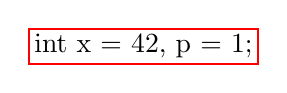
\begin{tikzpicture}\node[draw=red, thick, inner sep=2pt]{int x = 42, p = 1;};\end{tikzpicture}|

     for (int i = 1; i <= x; ++i)
     {    
          int y = i * i;
          p *= y;
     }
     std::cout << p << std::endl;
     
     return 0;
\end{consolethree}

As we enter the \texttt{for}-loop, we get a block of memory for the \texttt{for}-loop. Variable \texttt{i} in the \texttt{for}-loop resides in this block.

\begin{consolethree}[escapeinside=||]
#include <iostream>

int main()
{    
     int x = 42, p = 1;
     for (|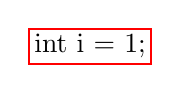
\begin{tikzpicture}\node[draw=red, thick, inner sep=2pt]{int i = 1;};\end{tikzpicture}| i <= x; ++i)
     {
         int y = i * i;
         p *= y;
     }
     std::cout << p << std::endl;

     return 0;
\end{consolethree}
\newpage
\sidenote
{
\begin{tikzpicture}
    \node[draw,text width=4cm,minimum height=7cm,minimum width=3cm, line width=0.05cm, inner sep=0.3cm,yshift=-3.5cm] (for3a) at (fora.south) {};
    \node[draw,text width=2cm,minimum height=1cm,line width=0.05cm,yshift=-8mm] (for3xbox) at (for3a.north){\normalsize{\texttt{\ \ \ \ \ \ \ \ \ }\textbf{42}}};
    \node[draw,text width=2cm,minimum height=1cm,line width=0.01cm,yshift=-8mm] (for3pbox) at (for3xbox.south){\normalsize{\texttt{\ \ \ \ \ \ \ \ \ }1}};
    
    \node[draw,yshift=-5mm,text width=2cm, line width=0.01cm, minimum height=1cm] (for3ibox) at (for3a.center) {\normalsize{\texttt{\ \ \ \ \ \ \ \ \ }1}};
    
    \node[draw,xshift=2mm,yshift=-9mm,text width=2cm, line width=0.01cm, minimum height=1cm] (for3ybox) at (for3ibox.south) {\normalsize{\texttt{\ \ \ \ \ \ \ \ \ }1}};
    
    \node[xshift=-2mm,draw,text width=2.9cm,line width=0.05cm,minimum height=1.5cm] (for3abox) at (for3ybox.center) {};
    \node[draw,yshift=-12mm,text width=3.5cm, line width=0.03cm,minimum height=3.8cm] (for3bbox) at (for3a.center) {};
    \node (forarranchor) at (for3abox.south) {};
    \node[xshift=-2mm] (for3inode) at (for3ibox.west){\normalsize{i}};
    \node[xshift=-2mm] (for3xnode) at (for3xbox.west){\normalsize{x}};
    \node[xshift=-2mm] (for3pnode) at (for3pbox.west){\normalsize{p}};
    \node[xshift=-2mm] (for3ynode) at (for3ybox.west){\normalsize{y}};
    \node[yshift=-10mm,xshift=-15mm,align=center] (for3memnode) at (for3a.south east){\normalsize{Memory of \textbf{body}}\\ \normalsize{of for-loop}};
    \draw[->,ultra thick] (for3memnode.north) to (forarranchor);

    \node[draw,yshift=-4cm,text width=4cm,minimum height=6cm,minimum width=3cm, line width=0.05cm, inner sep=0.3cm,yshift=-3.5cm] (for4a) at (for3a.south) {};
    \node[draw,text width=2cm,minimum height=1cm,line width=0.01cm,yshift=-8mm] (for4xbox) at (for4a.north){\normalsize{\texttt{\ \ \ \ \ \ \ \ \ }42}};
    \node[draw,text width=2cm,minimum height=1cm,line width=0.01cm,yshift=-8mm] (for4pbox) at (for4xbox.south){\normalsize{\texttt{\ \ \ \ \ \ \ \ \ }1}};
    \node[draw,yshift=-5mm,text width=2cm, line width=0.01cm, minimum height=1cm] (for4ibox) at (for4a.center) {\normalsize{\texttt{\ \ \ \ \ \ \ \ \ }1}}; 
    \node[draw,yshift=-12mm,text width=3.5cm, line width=0.03cm,minimum height=3cm] (for4bbox) at (for4a.center) {};
    \node[xshift=-2mm] (for4inode) at (for4ibox.west){\normalsize{i}};
    \node[xshift=-2mm] (for4xnode) at (for4xbox.west){\normalsize{x}};
    \node[xshift=-2mm] (for4pnode) at (for4pbox.west){\normalsize{p}};
\end{tikzpicture}
}
When we step into the body of the \texttt{for}-loop, we have \texttt{\textbf{another}} block. Variable \texttt{y} is created in this inner block:

\begin{consolethree}[escapeinside=||]
#include <iostream>

int main()
{    
     int x = 42, p = 1;
     for (int i = 1; i <= x; ++i)
     {    
          |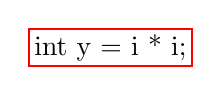
\begin{tikzpicture}\node[draw=red, thick, inner sep=2pt]{int y = i * i;};\end{tikzpicture}|
          p *= y;
     }
     std::cout << p << std::endl;

     return 0;
\end{consolethree}

When the last statement of the body of the \texttt{for}-loop is executed, we exit the body and variable \texttt{y} is destroyed:

\begin{consolethree}[escapeinside=||]
#include <iostream>

int main()
{    
     int x = 42, p = 1;

     for (int i = 1; i <= x; |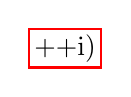
\begin{tikzpicture}\node[draw=red, thick, inner sep=2pt]{++i)};\end{tikzpicture}|
     {    
          int y = i * i;
          p *= y;
     }
     std::cout << p << std::endl;

     return 0;
\end{consolethree}

Of course when we enter the body of the \texttt{for}-loop the second time (when \texttt{i} = 2), variable \texttt{y} is created again.

Get it?
\newpage
And when we exit the \texttt{for}-loop altogether, variable \texttt{i} is destroyed because it is created in the \texttt{for}-loop:
\sidenote
{
\begin{tikzpicture}
    \node[draw,yshift=-4cm,text width=4cm,minimum height=6cm,minimum width=3cm, line width=0.05cm, inner sep=0.3cm,yshift=-3.5cm] (for4a) at (for3a.south) {};
    \node[draw,text width=2cm,minimum height=1cm,line width=0.01cm,yshift=-8mm] (for4xbox) at (for4a.north){\normalsize{\texttt{\ \ \ \ \ \ \ \ \ }42}};
    \node[draw,text width=2cm,minimum height=1cm,line width=0.01cm,yshift=-8mm] (for4pbox) at (for4xbox.south){\normalsize{\texttt{\ \ \ \ \ \ \ \ \ }1}};
    \node[xshift=-2mm] (for4xnode) at (for4xbox.west){\normalsize{x}};
    \node[xshift=-2mm] (for4pnode) at (for4pbox.west){\normalsize{p}};

    \node[draw,yshift=-12cm,text width=4cm,minimum height=6cm,minimum width=3cm, line width=0.05cm, inner sep=0.3cm,yshift=-3.5cm] (for5a) at (for3a.south) {};
    \node[draw,text width=2cm,minimum height=1cm,line width=0.01cm,yshift=-8mm] (for5xbox) at (for5a.north){\normalsize{\texttt{\ \ \ \ \ \ \ \ \ }42}};
    \node[draw,yshift=-15mm,xshift=3mm,text width=2cm,minimum height=1cm,line width=0.01cm,yshift=-8mm] (for5ybox) at (for5xbox.south){\normalsize{\texttt{\ \ \ \ \ \ \ \ \ }1}};
    \node[draw,text width=4cm,minimum height=2.5cm,minimum width=4cm, line width=0.05cm, yshift=-0.5cm] (for5a2) at (for5a) {};
    \node[draw,text width=3cm,minimum height=1.4cm,minimum width=3cm, line width=0.05cm] (for5ybox2) at (for5ybox) {};
    \node[xshift=-2mm] (for5xnode) at (for5xbox.west){\normalsize{x}};
    \node[xshift=-2mm] (for5ynode) at (for5ybox.west){\normalsize{y}};
    \node[yshift=1cm] (for5mainnode) at (for5a.north) {\normalsize{main}};
    \node[xshift=-1.5cm,yshift=-1cm] (for5whilenode) at (for5a.south) {\normalsize{while-loop}};
    \node[xshift=1.5cm,yshift=-1cm,align=center] (for5whilebdynode) at (for5a.south) {\normalsize{body of} \\\normalsize{while-loop}};
    \draw[ultra thick, ->] (for5mainnode.south) to (for5a.north);
    \draw[ultra thick, ->] (for5whilenode.north) to (for5a2.south);
    \draw[ultra thick, ->] (for5whilebdynode.north) to (for5ybox2.south);
\end{tikzpicture}
}

\begin{consolethree}[escapeinside=||]
#include <iostream>

int main()
{   
     int x = 42, p = 1;
     
     for (int i = 1; i <= x; ++i)
     {    
          int y = i * i;
          p *= y;
     }
     |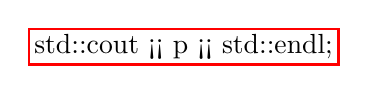
\begin{tikzpicture}\node[draw=red, thick, inner sep=2pt]{std::cout << p << std::endl;};\end{tikzpicture}|

     return 0;
\end{consolethree}

Note that variable \texttt{x} and \texttt{p} are still in scope; they are not destroyed.

What about the \texttt{while}-loop? The idea is similar: The \texttt{while}-loop has it' s memory and the body of the \texttt{while}-loop has an inner block.

\begin{consolethree}[escapeinside=||]
#include <iostream>

int main()
{    
     ...
     int x = 42;

     while (...)
     {     
           int y = 24;
           |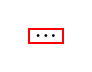
\begin{tikzpicture}\node[draw=red, thick, inner sep=2pt]{...};\end{tikzpicture}|
     }

     ...
}
\end{consolethree}

So remember this: each loop has it' s own memory for
variables and the body of the loop itself has its own memory.

\begin{ex} What is the problem? Fix it!

\begin{console}
std::cout << "Compute product of squares.";
std::cout << "Enter 0 to stop.\textbackslash n";

int prod = 1;
int x;
std::cin >> x;
while (x != 0)
{     
     int square = x * x;
     prod = prod * square;
     std::cout << "Product:" << prod << "\n";
     std::cin >> x;
}

std::cout << "\nProduct:" << prod << std::endl;
std::cout << "Last square: " << square
          << std::endl;
\end{console}
\end{ex}
If you need \textbf{several} temporary variables in a \texttt{for}-loop
you can do this:

\begin{consolethree}[escapeinside=||]
for (|\textbf{int i = 0, s = 5, t = 100}|; i < 10; i++)
{
    ...
}
\end{consolethree}

For instance if you want to print the running partial sums of summing 1
to 100 you can do this:

\begin{console}
for (int i = 0, s = 0; i < 10; i++)
{   
    s += i;
    std::cout << i << ' ' << s << '\n';
}
\end{console}

Of course note that in this case \texttt{s} is local to the \texttt{for}-loop and hence goes out of scope when the \texttt{for}-loop is done, i.e., it cannot be referenced outside the \texttt{for}-loop:

\begin{console}
for (int i = 0, s = 0; i < 10; i++)
{   
    s += i;
    std::cout << i << ' ' s << '\n';
}
std::cout << s << '\n'; // BADDDDDDDDDDDDD!!!!
\end{console}

\begin{ex}Can you also create variables in the header of an \texttt{if} statement? Can this work:

\begin{console}
int i = 0;

if (int x = i * i < 10)
{   

    ... do something with i and x ...

}
     ... do not use x!!! ...
\end{console}
\end{ex}
%\sectionthree{} requires solutions.tex, skipping for now
\newpage\EMPHASIZE{Variables with the same name}

Pay attention!!! This is something new!!!

You can actually create variables with the same name ... provided they
are either declared in non-overlapping blocks or one is defined in an
inner block.

Here' s the case where names are created in \EMPHASIZE{disjoint blocks}:

\begin{consolethree}[escapeinside=||]
...

for (int i = 0; i < 10; ++i)
{   
     int x, y, z;
     ...
}

|\tikzmarknode{disjointnode}{for (int i = 0; i < 100; ++i)}\sidebox{disjointbox}{No problem! You won't get a re-declaration because the previous i is already destroyed!}||\DrawArrow{disjointbox}{disjointnode}|
{   
     ...
     int y;

}

... 
\end{consolethree}

Do you see why there won' t be conflicts or confusion to C++?

Here' s the case where two names are created in \EMPHASIZE{nested blocks}:
\sidenote
{
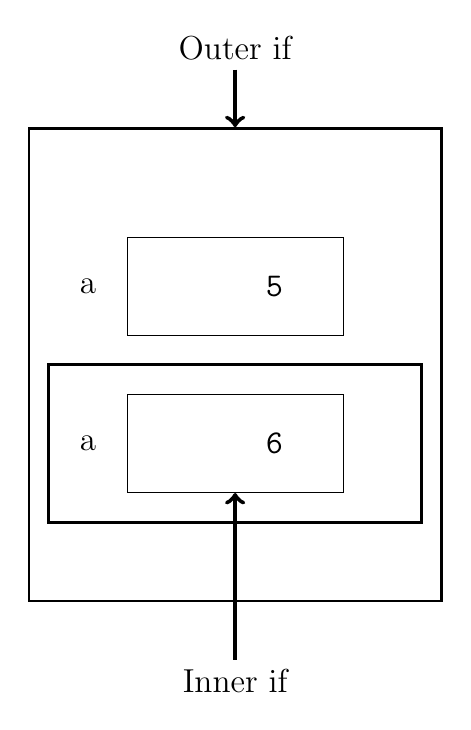
\begin{tikzpicture}
\node[draw, line width=1,text width=5cm, minimum height=6cm] (nestboxA) at (0,0) {};

\node[yshift=1cm,draw, line width=0.2,text width=2.5cm, minimum height=1.25cm] (nestboxB) at (nestboxA.center) {\large\texttt{\ \ \ \ \ \ \ \ \ \ \ \ \ \ 5}};

\node[yshift=-1cm,draw, line width=0.2,text width=2.5cm, minimum height=1.25cm] (nestboxC) at (nestboxA.center) {\large\texttt{\ \ \ \ \ \ \ \ \ \ \ \ \ \ 6}};

\node[draw, line width=1,text width=4.5cm, minimum height=2cm] (nestboxD) at (nestboxC.center) {};
\node[yshift=1cm] (nestouterif) at (nestboxA.north){\large{Outer if}};
\node[yshift=-1cm] (nestinnerif) at (nestboxA.south){\large{Inner if}};
\node[xshift=-5mm] (nestoutera) at (nestboxB.west) {\large{a}};
\node[xshift=-5mm] (nestinnera) at (nestboxC.west) {\large{a}};
\draw[ultra thick, ->] (nestouterif) to (nestboxA.north);
\draw[ultra thick, ->] (nestinnerif) to (nestboxC.south);
\end{tikzpicture}
}
\begin{console}
int x = 0, y = 0;
std::cin >> x >> y;

if (x == 0)
{    
     int a = 5;
     std::cout << a << std::endl;

     if (y == 1)
     {
          int a = 6;
          std::cout << a << std::endl;
     }
}
\end{console}

YIKES!!!

Note that the first print statement is not ambiguous. (Why?)

But what about the second? Which \texttt{a} is used in the second print statement???... go to next section to find out ...

WARNING: Although technically you can do the above (i.e. have two variables with the same name nest within blocks, it makes the code hard to read. Not only that, some languages do not allow this at all. Therefore you should \EMPHASIZE{AVOID DECLARING VARIABLES WITH THE SAME NAME IN NESTED BLOCKS}. The only \EMPHASIZE{exception} is a temporary (scratch) variable for instance like the counter variable of a \texttt{for}-loop

\begin{console}
for (int i = 0; i < 100; i++)
{    
     ...
     for (int i = -10; i < 10; i++)
     {    
          ...
     }
     ...
}
\end{console}

and only when the logic is easy to understand. But even then, you might still be shooting yourself in your foot later if you need to change the logic of your code.

\newpage\EMPHASIZE{How does C++ search for a variable?}

In looking for a variable C++ will always start from the block where the execution occurs. If the variable cannot be found, C++ will look for that variable in the nearest outer enclosing block.

Here's a simple example:
\sidenote
{
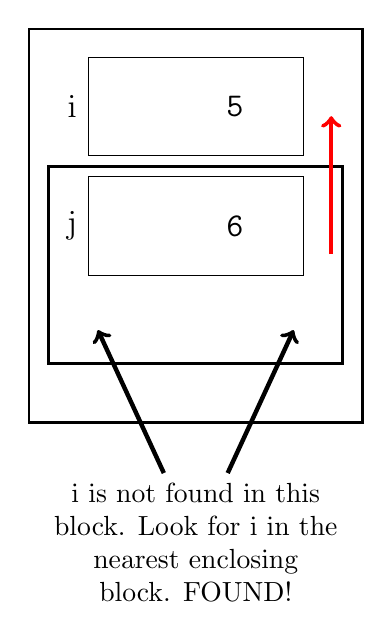
\begin{tikzpicture}
\node[draw, line width=1,text width=4cm, minimum height=5cm] (obbybox) at (0,4) {};
\node[yshift=-1cm,draw,line width=0.2,text width=2.5cm, minimum height=1.25cm] (obbybox5) at (obbybox.north) {\large\texttt{\ \ \ \ \ \ \ \ \ \ \ \ \ \ 5}};
\node[draw, line width=0.2,text width=2.5cm, minimum height=1.25cm] (obbybox6) at (obbybox.center) {\large\texttt{\ \ \ \ \ \ \ \ \ \ \ \ \ \ 6}};
\node[yshift=-0.5cm, draw, line width=1, text width=3.5cm, minimum height=2.5cm] (obby2box6) at (obbybox6.center) {};
\node[xshift=-2mm] (obbyj) at (obbybox5.west) {\large{i}};
\node[xshift=-2mm] (obbyi) at (obbybox6.west) {\large{j}};

\node[yshift=-1.5cm, align=center] (obbydesc) at (obbybox.south) {\normalsize{i is not found in this} \\ \normalsize{block. Look for i in the} \\ \normalsize{nearest enclosing}\\\normalsize{block. FOUND!}};
\node[xshift=0.35cm] (obbyredarrend) at (obbybox5.east){};
\node[xshift=0.35cm,yshift=-2cm] (obbyredarrstart) at (obbybox5.east){};
\node[xshift=-1.3cm,yshift=-1.2cm] (obbyboxend1) at (obbybox.center){};
\node[xshift=1.3cm,yshift=-1.2cm] (obbyboxend2) at (obbybox.center){};
\draw[ultra thick, ->] (obbydesc) to (obbyboxend1);
\draw[ultra thick, ->] (obbydesc) to (obbyboxend2);
\draw[ultra thick, ->, color=red] (obbyredarrstart) to (obbyredarrend);
\end{tikzpicture}
}


\begin{consolethree}[escapeinside=||]
#include <iostream>

int main()
{    
     int i = 5;

     if ( i > 0 )
     {    
          int j = 6;
          |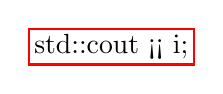
\begin{tikzpicture}\node[draw=red, thick, inner sep=2pt](nestconsolebox){std::cout << i;};\end{tikzpicture}|
     }

     return 0;
}
\end{consolethree}

\DrawArrowVH{obbybox.center}{nestconsolebox}


Of course C++ might need to search in several enclosing blocks before it's found.
\sidenote
{
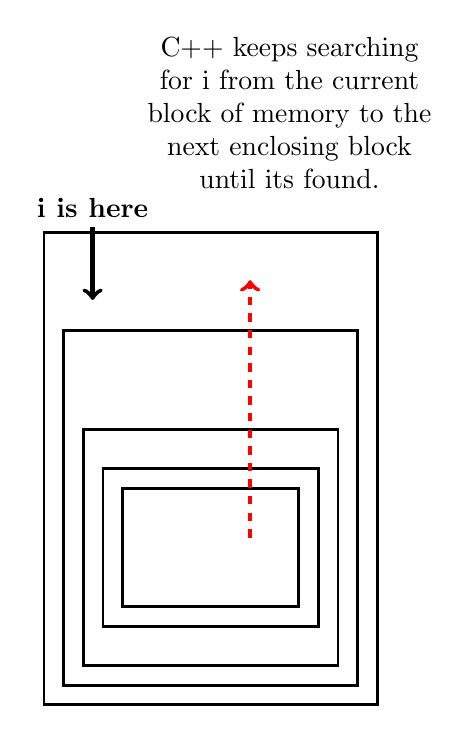
\begin{tikzpicture}
\node[draw,line width=1,text width=4cm, minimum height=6cm] (sbox) at (0,-2){};
\node[yshift=-0.5cm, draw, line width=1, text width=3.5cm, minimum height=4.5cm] (sbox1) at (sbox.center){};
\node[yshift=-0.5cm,draw, line width=1, text width=3cm, minimum height=3cm] (sbox2) at (sbox1.center){};
\node[draw, line width=1, text width=2.5cm, minimum height=2cm] (sbox3) at (sbox2.center){};
\node[draw, line width=1, text width=2cm, minimum height=1.5cm] (sbox4) at (sbox3.center){};
\node[xshift=0.5cm,yshift=-0.5cm] (sarrend) at (sbox.north){};
\node[xshift=0.5cm,yshift=-1cm] (sarrstart) at (sbox.center){};
\draw[line width=0.3, red, ultra thick, dashed, ->] (sarrstart) to (sarrend);
\node[xshift=1cm,yshift=1.5cm,align=center] (stxt) at (sbox.north){\normalsize{C++ keeps searching}\\ \normalsize{for i from the current}\\ \normalsize{block of memory to the}\\ \normalsize{next enclosing block}\\ \normalsize{until its found.}};
\node[xshift=-1.5cm,yshift=0.3cm,align=center] (stxti) at (sbox.north){\normalsize\textbf{i is here}};
\node[xshift=-1.5cm,yshift=-1cm] (sarrendi) at (sbox.north){};
\draw[line width=0.3, ultra thick, ->] (stxti.south) to (sarrendi);
\node[xshift=-5mm] (scons) at (stxti){};
\end{tikzpicture}
}
\begin{consolethree}[escapeinside=||]
#include <iostream>

int main()
{    
     int i = 5;
     while (i > 0)
     {    
          int j = 6;

          for (int k = 0; k < j; ++k)
          {   
               |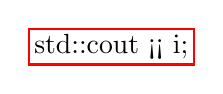
\begin{tikzpicture}\node[draw=red, thick, inner sep=2pt](csearchnode){std::cout << i;};\end{tikzpicture}|
          }
          --i;
     }
}
\end{consolethree}
\DrawArrow[dashed,red,ultra thick, -]{csearchnode}{scons}
\newpage
\begin{ex} Now look at the example from the previous section. Why is C++ not confused?
\sidenote
{
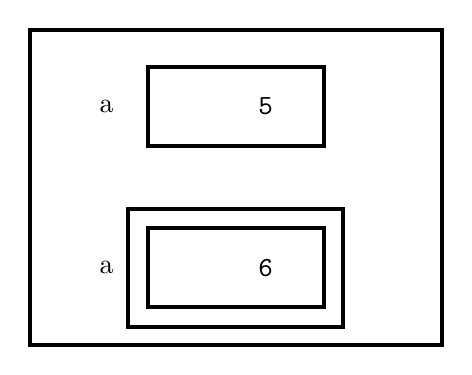
\begin{tikzpicture}
\node[draw,text width=5cm, minimum height=4cm, line width=0.05cm] (conbox){};
\node[yshift=-1cm,draw,text width=2cm, minimum height=1cm, line width=0.05cm] (conboxa) at (conbox.north){\normalsize\texttt{\ \ \ \ \ \ \ \ \ \ \ 5}};
\node[yshift=1cm,draw,text width=2cm, minimum height=1cm, line width=0.05cm] (conboxa2) at (conbox.south){\normalsize\texttt{\ \ \ \ \ \ \ \ \ \ \ 6}};
\node[draw,text width=2.5cm, minimum height=1.5cm, line width=0.05cm] (conboxa3) at (conboxa2.center){};
\node[xshift=-5mm] (conboxx) at (conboxa.west) {\normalsize{a}};
\node[xshift=-5mm] (conboxy) at (conboxa2.west) {\normalsize{a}};
\end{tikzpicture}
}
\begin{consolethree}[escapeinside=||]
int x = 0, y = 0;
std::cin >> x >> y;

if (x == 0)
{    
     int a = 5;
     std::cout << a << std::endl;
     if (y == 1)
     {    
          int a = 6;
          |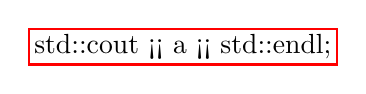
\begin{tikzpicture}\node[draw=red, thick, inner sep=2pt]{std::cout << a << std::endl;};\end{tikzpicture}|
     }
}
\end{consolethree}
\end{ex}
In this case when the variable \texttt{a} in the inner if-statement is created, we say that the innermost \texttt{a} \EMPHASIZE{hides} the outer \texttt{a}.

\begin{ex}
What is the output? (Or is there an error?)

\begin{console}
int x = 0, y = 1;

if (x == 0)
{    
     int a = 5;
     if (y == 1)
     {    
          std::cout << a << std::endl;
          int a = 6;
          std::cout << a << std::endl;
     }
}
\end{console}
\end{ex}

\begin{ex}
What is the output? (Or is there an error?)

\begin{console}
int x = 0, y = 1;

for (int x = 5; x < 10; x++)
{    
     std::cout << x << ' ' << y << std::endl;
     int y = 5;
     while (y > 0)
     {   
          int x = y + 1;
          std::cout << x << ' ' << y << std::endl;
          y++;
     }  
     std::cout << x << ' ' << y << std::endl;
}
\end{console}
\end{ex}

\begin{ex}
What is the output? (Or is there an error?)

\begin{console}
int i = 5, j = 6;
std::cout << i << ' ' << j << std::endl;
for (int i = 0; i < 3; i++)
{
      std::cout << i << ' ' << j << std::endl;
      if (i < j)
      {      
           std::cout << i << ' ' << j << std::endl;
           int i = 24;
           std::cout << i << ' ' << j << std::endl;
      }
      else
      {
           std::cout << i << ' ' << j << std::endl;
           int j = 42; 
           std::cout << i << ' ' << j << std::endl;
      }
      std::cout << i << ' ' << j << std::endl;
}
std::cout << i << ' ' << j << std::endl;
\end{console}
\end{ex}
\begin{ex}
What is the output? (Or is there an error?)

\begin{console}
int i = 5, j = 6;}
std::cout << i << ' ' << j << std::endl;
for (int i = 0; i < 3; i++)
{   
     int i = 8;
     std::cout << i << ' ' << j << std::endl;
     if (i < j)
     {
          std::cout << i << ' ' << j << std::endl;
          int i = 24; 
          std::cout << i << ' ' << j << std::endl;
     }
     else
     {
          std::cout << i << ' ' << j << std::endl;
          int j = 42;
          std::cout << i << ' ' << j << std::endl;
     }
     std::cout << i << ' ' << j << std::endl;
     int i = 9; 
}
std::cout << i << ' ' << j << std::endl;
\end{console}
\end{ex}
\newpage\EMPHASIZE{Principle of minimal scope}

Here's the principle of minimal scope:
\begin{center}
\EMPHASIZE{Keep the scope of variables}\\
\EMPHASIZE{as small as possible.}\\
\end{center}

(The above is suppose to blink).

For instance this is NOT GOOD:
\begin{console}
// compute the factorial of n
int i = 0;
int prod = 1;

int n = 0;
std::cin >> n;

for (i = 1; i <= n; i++)
{
    prod *= i;
}
std::cout << prod << std::endl;
\end{console}

This is BETTER

\begin{console}
// compute the factorial of n
int prod = 1;

int n = 0;
std::cin >> n;

for (int i = 1; i <= n; i++)
{    
     prod *= i;
}
std::cout << prod << std::endl;
\end{console}

\begin{ex} What's the difference?

Why? Frequently when you're solving a problem (not just a programming problem), you go through a sequence of steps of computation or transformation on the data. Each step usually requires some input data to modify something (such as a variable) or to perform a task (such as printing something to the screen in a game).
\end{ex}
For our program above you should be able to see these steps:

\begin{python}
from latextool_basic import *
p = Plot()
#p += Grid(x0=-4,y0=-4,x1=4,y1=4)

B1 = Rect(-2,2,2,3,label=r'Prompt user for n',linewidth=0.05)
B2 = Rect(-4,-1,4,0,label=r'Compute factorial of n and store in prod',linewidth=0.05)
B3 = Rect(-2,-4,2,-3,label=r'Print prod',linewidth=0.05)

p += B1
p += B2
p += B3
p += Line(points=[(0,5),(0,3)], linewidth=0.1, endstyle='>')
p += Line(points=[(0,2),(0,0)], linewidth=0.1, endstyle='>')
p += Line(points=[(0,-1),(0,-3)], linewidth=0.1, endstyle='>')
p += Line(points=[(0,-4),(0,-6)], linewidth=0.1, endstyle='>')

print(p)
\end{python}

A well-written program will always try to minimize the inputs and
outputs (or change) within a step such as this:
\begin{python}
from latextool_basic import *
p = Plot()
#p += Grid(x0=-4,y0=-4,x1=4,y1=4)
B2 = Rect(-4,-1,4,0,label=r'Compute factorial of n and store in prod',linewidth=0.05)
p += B2
p += Line(points=[(0,2),(0,0)], linewidth=0.1, endstyle='>')
p += Line(points=[(0,-1),(0,-3)], linewidth=0.1, endstyle='>')
print(p)
\end{python}

Why? Because the more stuff you have in a step the more complex it will be. That means that the code is harder to read, debug, and maintain for future change. In the real world, software engineers write new code and maintain code base (maintain = correct, add and delete). Now look at this:

\begin{python}
from latextool_basic import *
p = Plot()
#p += Grid(x0=-4,y0=-4,x1=4,y1=4)
B2 = Rect(-4,-1,4,0,label=r'Compute factorial of n and store in prod',linewidth=0.05)
p += B2
p += Line(points=[(0,2),(0,0)], linewidth=0.1, endstyle='>')
p += Line(points=[(0,-1),(0,-3)], linewidth=0.1, endstyle='>')
print(p)
\end{python}

What variables are involved in this step? Don't think about the internals of this chunk of code. Think of the code as a black box. You need n (that's the input) and you want to compute the factorial of n (that's the output) and you want to put that value in to prod (that's the transformation).

So two variables take part in this step.

Now look at the code from the first program (the part in bold):

\begin{consolethree}[escapeinside=||]
// compute the factorial of n
int i = 0;
int prod = 1;

int n = 0;
std::cin >> n;

|\textbf{for (i = 1; i <= n; i++)}|
|\textbf{\{}|
    |\textbf{prod *= i;}|
|\textbf{\}}|

std::cout << prod << std::endl; 
\end{consolethree}

You see clearly that besides ``sending in'' variables \texttt{n} and \texttt{prod} to this step, \underline{\textbf{you also ``send in'' variable }\textbf{i}}.

Now look at the improved version:

\begin{consolethree}[escapeinside=||]
// compute the factorial of n
int prod = 1;

int n = 0;
std::cin >> n;

|\textbf{for (int i = 1; i <= n; i++)}|
|\textbf{\{}|
    |\textbf{prod *= i;}|
|\textbf{\}}|

std::cout << prod << std::endl; 
\end{consolethree}

Variable \texttt{i} is internal to the step that computes the factorial of \texttt{n} and stores it in \texttt{prod}. Outside the code that computes and stores the factorial of \texttt{n} in \texttt{prod}, variable \texttt{i} does not exist.

Get it?

This also prevent ``side effects'' in code. (I've already mentioned this.) If a variable has a large scope, and you modify it in some place, it might have unexpected effects. Here's something similar to a previous example -- it's important enough to repeat!!! For instance suppose work in a team and you're given this code segment:

\begin{console}
...
int i = 42;
...
for (; i < 100; i++)
{
    ...
}
.... 
\end{console}

where you expect the \texttt{for}-loop to run from \texttt{i} = 42 to \texttt{i} = 99. One of your colleagues might see the variable \texttt{i} and add some code like so:

\begin{console}
...
int i = 42;
...
for (i = 1000; i > 0; --i)
{    
     ...
}
...
for (; i < 100; i++)
{     
     ...
}
.... 
\end{console}

So guess what? When you use \texttt{i}, the initial value for you is now 0 and not 42 and your program doesn't work anymore. Tough. What's worse is when you try to debug, you might not even see it because you kept saying to yourself ``But, but, but ... I didn't change anything ever since it was working!!! ... and my code looks the same as before!!!''

This is one of the most important reasons why we also try to restrict the scope of a variable. If it's meant to be a ``scratch'' variable, then create it in such a way that it gets destroy ASAP.

As you can see from the example, one way to minimize scopes is to declare only when you need to and in the \EMPHASIZE{innermost block} whenever possible. For our example, we declare \texttt{i} within the for-loop block.

\EMPHASIZE{NOTE: }Some people declare all variables at the beginning of a function. That's because \underline{\textbf{some}} programming languages specify that \underline{\textbf{all}} declaration statements must come before other types of statements.
That's not the case for C++ or other modern programming languages.

Now let's go back to that program again. There's one other spot where you can minimize the scope of a variable.

\begin{consolethree}[escapeinside=||]
// compute the factorial of n
|\textbf{int prod = 1;}|

int n = 0;
std::cin >> n;

for (int i = 1; i <= n; i++)
{    
     prod *= i;
}

std::cout << prod << std::endl;
\end{consolethree}

Note that \texttt{prod} is not used until the \texttt{for}-loop. So you can
write this:

\begin{consolethree}[escapeinside=||]
// compute the factorial of n
int n = 0;
std::cin >> n;

|\textbf{int prod = 1;}|
for (int i = 1; i <= n; i++)
{    
     prod *= i;
}
std::cout << prod << std::endl;
\end{consolethree}

This however is \textbf{not as crucial} as the previous change because \texttt{prod} is not destroyed. Furthermore \texttt{prod} is part of the larger goal of computing the factorial. Hence it's OK to declare \texttt{prod} early so that readers of your code can see it early, especially if you mention \texttt{prod} in your comments like this:

\begin{consolethree}[escapeinside=||]
// compute the factorial of n and store it in prod
int n = 0;
|\textbf{int prod = 1;}|

std::cin >> n;

for (int i = 0; i <= n; i++)
{    
     prod *= i;
}

std::cout << prod << std::endl;
\end{consolethree}

See that?

\begin{ex} Rewrite the following program so that variables have minimal scopes.

\begin{console}
#include <iostream>

int main()
{   
     int answer, i, first, last, sum, term;
     std::cout << "Find sum? (1 -- yes or 0 - no) ";
     std::cin >> answer;
     
     if (answer == 1)
     {    
          std::cout << "First int:";
          std::cin >> first;
          std::cout << "Last int:"
          std::cin >> last;

          sum = 0;
          for (i = first; i <= last; ++i)
          {    
               term = i * i * i * i;
               sum += term;
          }
          std::cout << "Sum:" << sum << std::endl;
     }

     return 0;
}
\end{console}

\end{ex}



\begin{ex} The following program computes the sum
\begin{center}
(1/1) + (1/1)(1/2) + (1/1)(1/2)(1/3) + (1/1)(1/2)(1/3)(1/4) + ...
\end{center}
(that's in mathematical notation and not C++ notation)
where the number of terms is specified by the user. Verify by hand that it does not work correctly. Explain why and correct the program; there are several problems.


\begin{console}
int n = 0, i = 0, j = 0, term = 0, sum = 0;

std::cin >> n;

for (i = 1; i <= n; ++i)
{    
     // Compute i-th term, i.e. 1/1*...*1/i
     for (j = 0; j < i; ++j)
     {    
          term *= 1.0 / j;
     }

     // Accumulate term into sum by addition
     sum += term;
}

std::cout << sum << std::endl;
\end{console}
\end{ex}
\newpage\EMPHASIZE{Summary}
The scope of a variable is where the variable can be accessed. This is
from the declaration of the variable to the end of the block where it is
declared.


%reminder to tell dr liow to update the documentation for the 'verbatim' section to change the example of frame=None to frame='none' 
\begin{python}
from latextool_basic import *
from latexcircuit import *
p = Plot()
#p += Grid(x0=-4,y0=-4,x1=4,y1=4)
t0 = POINT(x=-4,y=3,label=r'\texttt{...}',r=0)
t1 = POINT(x=-4.5,y=2.4,label=r'\texttt{%s}' % '\{',r=0)
t2 = POINT(x=-3,y=1.8,label=r'\texttt{     ...}',r=0)
t3 = POINT(x=0.1,y=1.2,label=r'\texttt{     double i = 0.0;}',r=0)
t4 = POINT(x=-3,y=0.6,label=r'\texttt{     ...}',r=0)
t5 = POINT(x=-4.5,y=0,label=r'\texttt{%s}' % '\}',r=0)
t6 = POINT(x=-4,y=-0.6,label=r'\texttt{...}',r=0)
p += str(t0)
p += str(t1)
p += str(t2)
p += str(t3)
p += str(t4)
p += str(t5)
p += str(t6)
p += Rect(2,-0.6,8,3,linewidth=0.15)
p += Rect(2.5,0,7.5,2.5,linewidth=0.15)
p += Rect(3.5,0.5,6.5,2,linewidth=0.05)
p += Rect(3.1,1.1,3.1,1.1,linewidth=0,label=r'i')
print(p)
\end{python}
If a variable name is used in two declarations, then the two blocks
where they are declared do not overlap or one is nested within the
other.

\begin{python}
from latextool_basic import *
p = Plot()
#p += Grid(x0=-4,y0=-4,x1=4,y1=4)
p += Rect(2,-3,8,3,linewidth=0.15)
p += Rect(-6,-3,0,3,linewidth=0.15)
p += Rect(2.5,-2.5,7.5,2.5,linewidth=0.15)

p += Rect(3,-2.3,7,-0.1,linewidth=0.15)
p += Rect(3.5,0.5,6.5,2,linewidth=0.05)
p += Rect(3.5,-2,6.5,-0.5,linewidth=0.05)
p += Rect(3.25,-1.45,3.25,-1.45,linewidth=0,label=r'i')
p += Rect(3.25,1.3,3.25,1.3,linewidth=0,label=r'i')

p += Rect(-5.5,0,-0.5,2.5,linewidth=0.15)
p += Rect(-4.5,0.5,-1.5,2,linewidth=0.05)
p += Rect(-4.7,1.3,-4.7,1.3,linewidth=0,label=r'i')

p += Rect(-5.5,-2.5,-0.5,-0.2,linewidth=0.15)
p += Rect(-4.5,-2,-1.5,-0.5,linewidth=0.05)
p += Rect(-4.7,-1.45,-4.7,-1.45,linewidth=0,label=r'i')

print(p)
\end{python}
If the program tries to access a variable and it's not found in the current block, then the program will look for the variable in the \texttt{\textbf{nearest}} outer block.

\begin{python}
from latextool_basic import *
p = Plot()
#p += Grid(x0=0,y0=-4,x1=10,y1=4)
D = '''
Program execution in
this block and looks for
i. Program will keep
looking in the next outer
block until it's found or
if not, we have an error
'''
code(p, D)
p += Rect(7,-3,13,3,linewidth=0.15)
p += Rect(7.5,-2.5,12.5,0.1,linewidth=0.15)
p += Rect(8.5,0.5,11.5,2,linewidth=0.05)
p += Rect(8.5,-2,11.5,-0.5,linewidth=0.05)
#p += Rect(8.25,-1.45,8.25,-1.45,linewidth=0,label=r'i')
p += Rect(8.25,1.3,8.25,1.3,linewidth=0,label=r'i')
p += Circle(x=10,y=-1.2,r=0.5, linecolor='red',background='red')
p += Line(points=[(10,-1.2),(10,0.3)],endstyle='>',linewidth=0.1,linecolor='red',linestyle='dashed')
print(p)
\end{python}
The \texttt{for}-loop and \texttt{while}-loop create a block and their bodies create a block within the loop's block.
